\documentclass[a4paper,12pt]{article}
\usepackage[utf8]{inputenc}
\usepackage{geometry}
\usepackage{fancyhdr}
\usepackage{listings}
\usepackage{xcolor}
\usepackage{graphicx}
\usepackage{float}
\usepackage{hyperref} % Added for clickable links

% Hyperlink configuration
\hypersetup{
    colorlinks=true,
    linkcolor=blue, % Makes the clickable links blue
    filecolor=magenta,      
    urlcolor=cyan,
    pdftitle={Assignment 4},
}

% Margins
\geometry{left=15mm, right=15mm, top=25mm, bottom=15mm}

% Header/Footer
\pagestyle{fancy}
\fancyhf{}
\renewcommand{\headrulewidth}{0pt}
\rfoot{Page \thepage}

\fancypagestyle{firstpage}{
    \fancyhf{}
    \lhead{
        \small \textbf{Name:} Mrigaj Shaw \\ 
        \small \textbf{Roll No:} 2024CSB041
    }
    \chead{\LARGE \textbf{Assignment 4}} 
    \rfoot{Page \thepage}
    \renewcommand{\headrulewidth}{1pt}
}

% Code Style
\definecolor{codegreen}{rgb}{0,0.6,0}
\definecolor{codegray}{rgb}{0.5,0.5,0.5}
\definecolor{codepurple}{rgb}{0.58,0,0.82}
\definecolor{backcolour}{rgb}{0.95,0.95,0.92}

\lstdefinestyle{MyCodeStyle}{
    backgroundcolor=\color{backcolour},   
    commentstyle=\color{codegreen},
    keywordstyle=\color{magenta},
    numberstyle=\tiny\color{codegray},
    stringstyle=\color{codepurple},
    basicstyle=\ttfamily\footnotesize,
    breakatwhitespace=false,         
    breaklines=true,                 
    keepspaces=true,                 
    numbers=left,                    
    numbersep=5pt,                  
    showspaces=false,                
    showstringspaces=false,
    showtabs=false,                  
    tabsize=4
}
\lstset{style=MyCodeStyle}

\begin{document}
\thispagestyle{firstpage}

% --- Problem1 ---
\section*{Problem 1}
\textbf{Problem Statement:} Write a C program to represent and analyze two real-world networks using \textbf{graph data structures}, where one graph is \textbf{sparse} and the other is \textbf{dense}. Let the number of vertices be $n = 100$. For the sparse graph, take the number of edges as $e_s = 120$, such that
$$e_s \ll \frac{n(n - 1)}{2},$$
and generate the edges \textbf{randomly}. Represent this sparse graph using an \textbf{adjacency list} for both \textbf{unweighted edges} (showing only connections) and \textbf{weighted edges} (assigning a random cost or distance to each edge).

For the dense graph, take the number of edges as $e_d = 4500$, such that
$$e_d \approx \frac{n(n - 1)}{2},$$
and generate the edges \textbf{randomly}. Represent this dense graph using an \textbf{adjacency matrix} for both \textbf{unweighted and weighted edges}. The program should \textbf{automatically generate random vertex pairs and edge weights}, construct the corresponding graph representations, and \textbf{display the adjacency list and adjacency matrix}.
\subsection*{Code}
\lstinputlisting[language=C]{Problem1/RepresentationsOfGraph.c}
\subsection*{Output}
\begin{figure}[H]
    \centering
    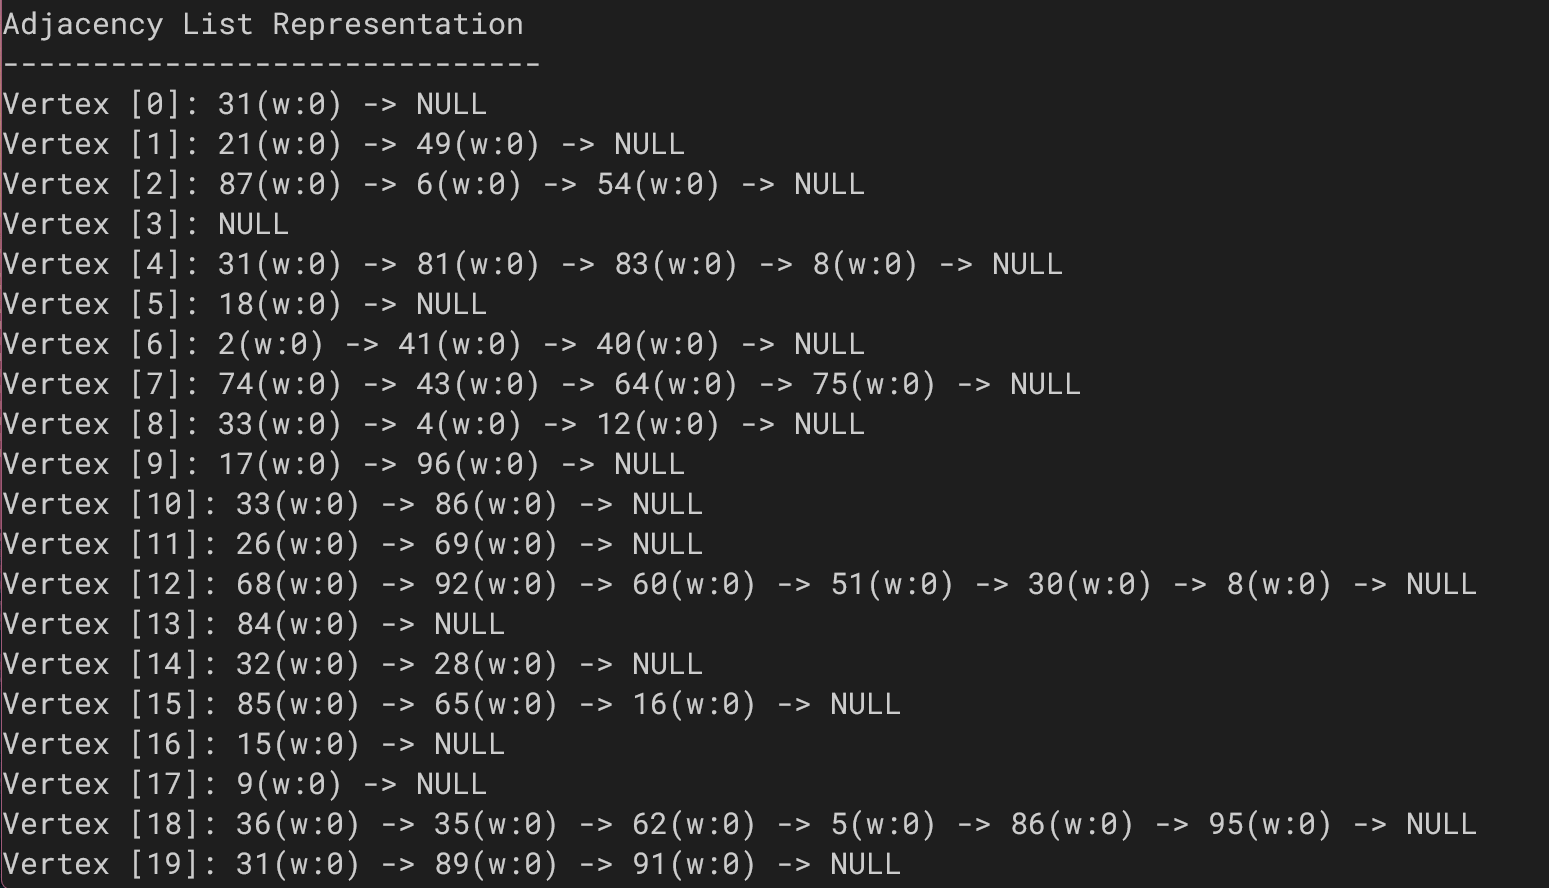
\includegraphics[width=0.9\textwidth]{Problem1/Problem1_1.png}
\end{figure}
\begin{figure}[H]
    \centering
    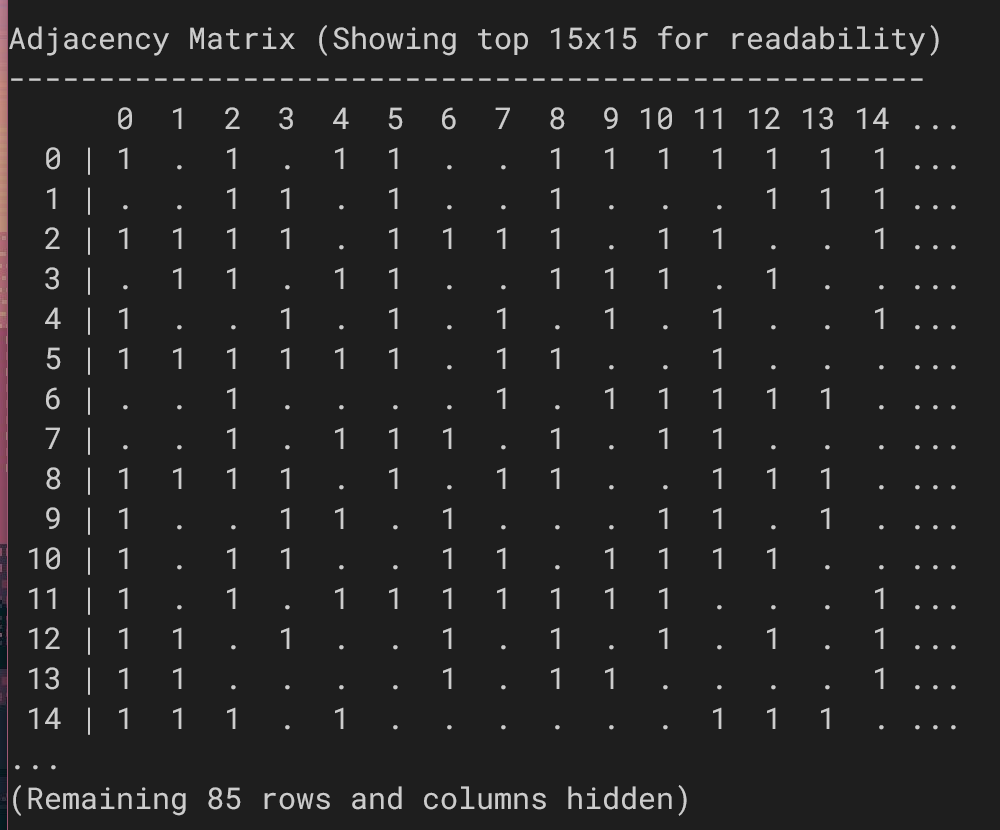
\includegraphics[width=0.9\textwidth]{Problem1/Problem1_2.png}
\end{figure}
\subsection*{Inference}
\begin{itemize}
    \item The graph was successfully implemented using both Adjacency List and Adjacency Matrix representations.
    \item The \textbf{Adjacency List} requires $O(V + E)$ space, making it highly efficient for sparse graphs.
    \item The \textbf{Adjacency Matrix} requires $O(V^2)$ space, which is optimal for dense graphs and $O(1)$ edge-lookups, but wastes memory for sparse networks.
    \item \textit{Note: The core \hyperlink{target:adjlist}{\texttt{AdjacencyList.h}} header was implemented from scratch and serves as the foundational data structure utilized across all subsequent graph problems in this assignment.}
\end{itemize}

\newpage

% --- Problem2 ---
\section*{Problem 2}
\textbf{Problem Statement:} Write a C program to connect 6 cities (C1--C6) with minimum cost using \textbf{Prim's Algorithm} and a \textbf{Min-Priority Queue}. The cost of connecting each pair of cities (in lakhs) is:

\begin{center}
\begin{tabular}{rll}
$(C1, C2) = 3,$ & $(C1, C3) = 1,$ & $(C1, C4) = 6,$ \\
$(C2, C3) = 5,$ & $(C2, C5) = 3,$ & $(C3, C4) = 5,$ \\
$(C3, C6) = 4,$ & $(C4, C6) = 2,$ & $(C5, C6) = 6$
\end{tabular}
\end{center}

Your program should:
\begin{enumerate}
    \item Represent the graph using an \textbf{adjacency list}.
    \item Implement \textbf{Prim's Algorithm} starting from vertex C1 using a \textbf{Min-Priority Queue}.
    \item Display the edges in the \textbf{Minimum Spanning Tree (MST)}, the \textbf{total minimum cost}, and the \textbf{order of vertices added}.
\end{enumerate}
\subsection*{Code}
\lstinputlisting[language=C]{Problem2/primsAlgorithm.c}
\subsection*{Output}
\begin{figure}[H]
    \centering
    
\includegraphics[width=0.9\textwidth]{Problem2/Problem2.png}
\end{figure}
\subsection*{Inference}
\begin{itemize}
    \item Prim's algorithm was implemented using the Adjacency List and a custom \hyperlink{target:minheap}{\texttt{MinHeap.h}} Min-Priority Queue (see Appendix).
    \item The overall time complexity is \textbf{$O(E \log V)$} because extracting the minimum weight edge from the heap takes $O(\log V)$ time, performed for up to $E$ edges in the worst case.
    \item A boolean \texttt{visited} array was utilized alongside a "lazy" heap approach.
    \item This efficiently ignores stale edges and prevents the formation of cycles during the Minimum Spanning Tree (MST) construction.
\end{itemize}

\newpage

% --- Problem3 ---
\section*{Problem 3}
\textbf{Problem Statement:} Write a C program to connect 6 cities (C1--C6) with minimum cost using \textbf{Kruskal's Algorithm}. The cost of connecting each pair of cities (in lakhs) is:

\begin{center}
\begin{tabular}{rll}
$(C1, C2) = 3,$ & $(C1, C3) = 1,$ & $(C1, C4) = 6,$ \\
$(C2, C3) = 5,$ & $(C2, C5) = 3,$ & $(C3, C4) = 5,$ \\
$(C3, C6) = 4,$ & $(C4, C6) = 2,$ & $(C5, C6) = 6$
\end{tabular}
\end{center}

Your program should:
\begin{enumerate}
    \item Represent the graph using an \textbf{edge list}.
    \item Sort all edges in ascending order and construct the \textbf{Minimum Spanning Tree (MST)} using \textbf{Union-Find (Disjoint Set)} to prevent cycles.
    \item Display the edges included in the MST, the \textbf{total minimum cost}, and the \textbf{order in which edges are added}.
\end{enumerate}
\subsection*{Code}
\lstinputlisting[language=C]{Problem3/KruskallsAlgorithm.c}
\subsection*{Output}
\begin{figure}[H]
    \centering
    
\includegraphics[width=0.9\textwidth]{Problem3/Problem3.png}
\end{figure}
\subsection*{Inference}
\begin{itemize}
    \item Kruskal's algorithm was implemented by extracting a flat array of unique edges from the undirected Adjacency List.
    \item Edges were sorted in ascending order using Quicksort, dictating the overall \textbf{$O(E \log E)$} time complexity.
    \item Cycle detection was handled efficiently using a custom \hyperlink{target:dsu}{\texttt{DisjointSetUnion.h}} (see Appendix) featuring both path compression and union by rank.
    \item The near $O(1)$ time complexity of these Union-Find operations ensures they do not bottleneck the primary sorting phase.
\end{itemize}

\newpage

% --- Problem4 ---
\section*{Problem 4}
\textbf{Problem Statement:} Write a C program to compute the \textbf{Minimum Spanning Tree (MST)} of a large-scale \textbf{smart city power distribution network} consisting of two independent weighted graphs $G_1(V_1, E_1)$ and $G_2(V_2, E_2)$, interconnected by a \textbf{single high-capacity transmission edge} having the \textbf{maximum weight among all edges}. This high-weight edge must always be included in the final MST. Apply \textbf{Kruskal's algorithm} on graph $G_1$, considering it as a \textbf{sparse graph}, and apply \textbf{Prim's algorithm} on graph $G_2$, considering it as a \textbf{dense graph}. After computing the MSTs of both graphs separately, merge them using the \textbf{mandatory high-weight edge} to construct the \textbf{global MST} of the combined network. The program should take the number of vertices, edges, and weighted edge lists as input, compute the \textbf{final MST}, display the \textbf{selected edges}, and output the \textbf{total cost} of the spanning tree.
\subsection*{Code}
\lstinputlisting[language=C]{Problem4/SmartCityPowerDistribution.c}
\subsection*{Output}
\begin{figure}[H]
    \centering
    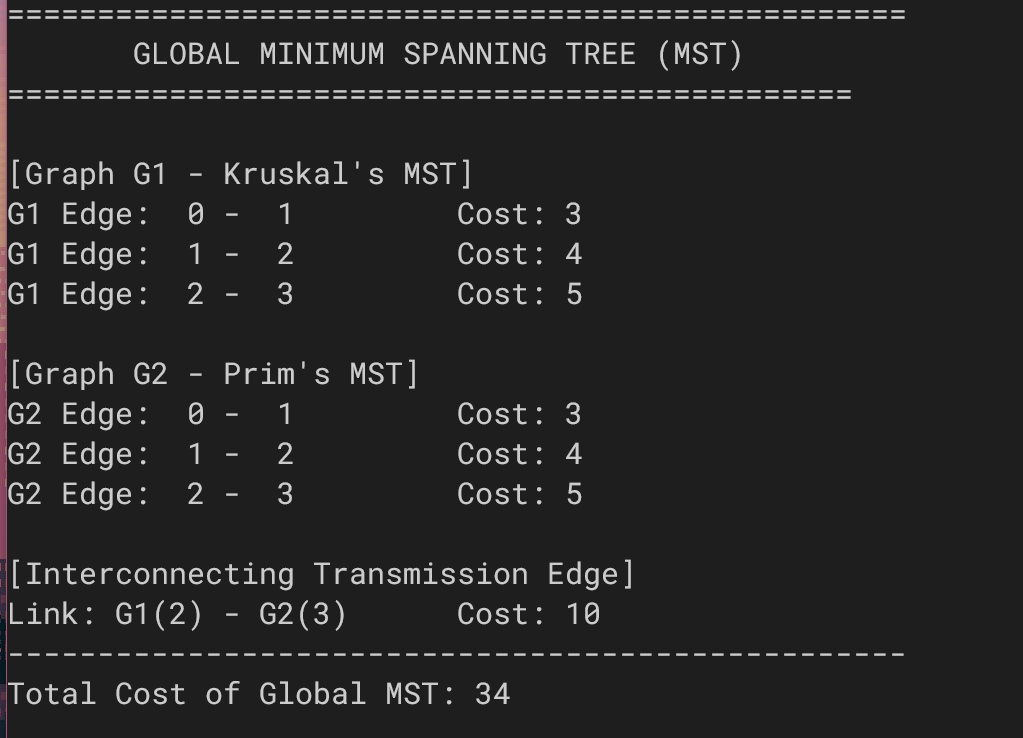
\includegraphics[width=0.9\textwidth]{Problem4/Problem4.png}
\end{figure}
\subsection*{Inference}
\begin{itemize}
    \item This hybrid problem effectively leverages the distinct architectural strengths of both MST algorithms.
    \item \textbf{Kruskal's algorithm} is optimally applied to the sparse graph ($G_1$) as sorting a small edge list is highly efficient ($O(E_1 \log E_1)$).
    \item \textbf{Prim's algorithm} is applied to the dense graph ($G_2$), where its $O(E_2 \log V_2)$ complexity natively handles heavy interconnections without requiring a massive global array sort.
    \item Connecting the two independently generated MSTs via the single mandatory high-capacity transmission edge acts as a bridge.
    \item This final connection takes $O(1)$ time and mathematically guarantees a valid, globally optimal MST for the combined smart city network.
\end{itemize}

\newpage

% --- Appendix ---
\section*{Appendix: Shared Data Structures}
The following header files were implemented from scratch and utilized across multiple problems in this assignment to handle graph and priority operations efficiently.

\vspace{0.5cm}

\hypertarget{target:minheap}{} 
\subsection*{1. Min-Priority Queue (\texttt{MinHeap.h})}
\lstinputlisting[language=C]{./MinHeap/MinHeap.h} 

\vspace{1cm}

\newpage

\hypertarget{target:dsu}{} 
\subsection*{2. Disjoint Set Union (\texttt{DisjointSetUnion.h})}
\lstinputlisting[language=C]{../Assignment_5/DisjointSetUnion/DisjointSetUnion.h} 

\vspace{1cm}

\newpage
\hypertarget{target:adjlist}{} 
\subsection*{3. Adjacency List (\texttt{AdjacencyList.h})}
\lstinputlisting[language=C]{./AdjacencyList/AdjacencyList.h} % Note: Adjust this path if your folder structure is different!

\end{document}